\documentclass[1p]{elsarticle_modified}
%\bibliographystyle{elsarticle-num}

%\usepackage[colorlinks]{hyperref}
%\usepackage{abbrmath_seonhwa} %\Abb, \Ascr, \Acal ,\Abf, \Afrak
\usepackage{amsfonts}
\usepackage{amssymb}
\usepackage{amsmath}
\usepackage{amsthm}
\usepackage{scalefnt}
\usepackage{amsbsy}
\usepackage{kotex}
\usepackage{caption}
\usepackage{subfig}
\usepackage{color}
\usepackage{graphicx}
\usepackage{xcolor} %% white, black, red, green, blue, cyan, magenta, yellow
\usepackage{float}
\usepackage{setspace}
\usepackage{hyperref}

\usepackage{tikz}
\usetikzlibrary{arrows}

\usepackage{multirow}
\usepackage{array} % fixed length table
\usepackage{hhline}

%%%%%%%%%%%%%%%%%%%%%
\makeatletter
\renewcommand*\env@matrix[1][\arraystretch]{%
	\edef\arraystretch{#1}%
	\hskip -\arraycolsep
	\let\@ifnextchar\new@ifnextchar
	\array{*\c@MaxMatrixCols c}}
\makeatother %https://tex.stackexchange.com/questions/14071/how-can-i-increase-the-line-spacing-in-a-matrix
%%%%%%%%%%%%%%%

\usepackage[normalem]{ulem}

\newcommand{\msout}[1]{\ifmmode\text{\sout{\ensuremath{#1}}}\else\sout{#1}\fi}
%SOURCE: \msout is \stkout macro in https://tex.stackexchange.com/questions/20609/strikeout-in-math-mode

\newcommand{\cancel}[1]{
	\ifmmode
	{\color{red}\msout{#1}}
	\else
	{\color{red}\sout{#1}}
	\fi
}

\newcommand{\add}[1]{
	{\color{blue}\uwave{#1}}
}

\newcommand{\replace}[2]{
	\ifmmode
	{\color{red}\msout{#1}}{\color{blue}\uwave{#2}}
	\else
	{\color{red}\sout{#1}}{\color{blue}\uwave{#2}}
	\fi
}

\newcommand{\Sol}{\mathcal{S}} %segment
\newcommand{\D}{D} %diagram
\newcommand{\A}{\mathcal{A}} %arc


%%%%%%%%%%%%%%%%%%%%%%%%%%%%%5 test

\def\sl{\operatorname{\textup{SL}}(2,\Cbb)}
\def\psl{\operatorname{\textup{PSL}}(2,\Cbb)}
\def\quan{\mkern 1mu \triangleright \mkern 1mu}

\theoremstyle{definition}
\newtheorem{thm}{Theorem}[section]
\newtheorem{prop}[thm]{Proposition}
\newtheorem{lem}[thm]{Lemma}
\newtheorem{ques}[thm]{Question}
\newtheorem{cor}[thm]{Corollary}
\newtheorem{defn}[thm]{Definition}
\newtheorem{exam}[thm]{Example}
\newtheorem{rmk}[thm]{Remark}
\newtheorem{alg}[thm]{Algorithm}

\newcommand{\I}{\sqrt{-1}}
\begin{document}

%\begin{frontmatter}
%
%\title{Boundary parabolic representations of knots up to 8 crossings}
%
%%% Group authors per affiliation:
%\author{Yunhi Cho} 
%\address{Department of Mathematics, University of Seoul, Seoul, Korea}
%\ead{yhcho@uos.ac.kr}
%
%
%\author{Seonhwa Kim} %\fnref{s_kim}}
%\address{Center for Geometry and Physics, Institute for Basic Science, Pohang, 37673, Korea}
%\ead{ryeona17@ibs.re.kr}
%
%\author{Hyuk Kim}
%\address{Department of Mathematical Sciences, Seoul National University, Seoul 08826, Korea}
%\ead{hyukkim@snu.ac.kr}
%
%\author{Seokbeom Yoon}
%\address{Department of Mathematical Sciences, Seoul National University, Seoul, 08826,  Korea}
%\ead{sbyoon15@snu.ac.kr}
%
%\begin{abstract}
%We find all boundary parabolic representation of knots up to 8 crossings.
%
%\end{abstract}
%\begin{keyword}
%    \MSC[2010] 57M25 
%\end{keyword}
%
%\end{frontmatter}

%\linenumbers
%\tableofcontents
%
\newcommand\colored[1]{\textcolor{white}{\rule[-0.35ex]{0.8em}{1.4ex}}\kern-0.8em\color{red} #1}%
%\newcommand\colored[1]{\textcolor{white}{ #1}\kern-2.17ex	\textcolor{white}{ #1}\kern-1.81ex	\textcolor{white}{ #1}\kern-2.15ex\color{red}#1	}

{\Large $\underline{12n_{0585}~(K12n_{0585})}$}

\setlength{\tabcolsep}{10pt}
\renewcommand{\arraystretch}{1.6}
\vspace{1cm}\begin{tabular}{m{100pt}>{\centering\arraybackslash}m{274pt}}
\multirow{5}{120pt}{
	\centering
	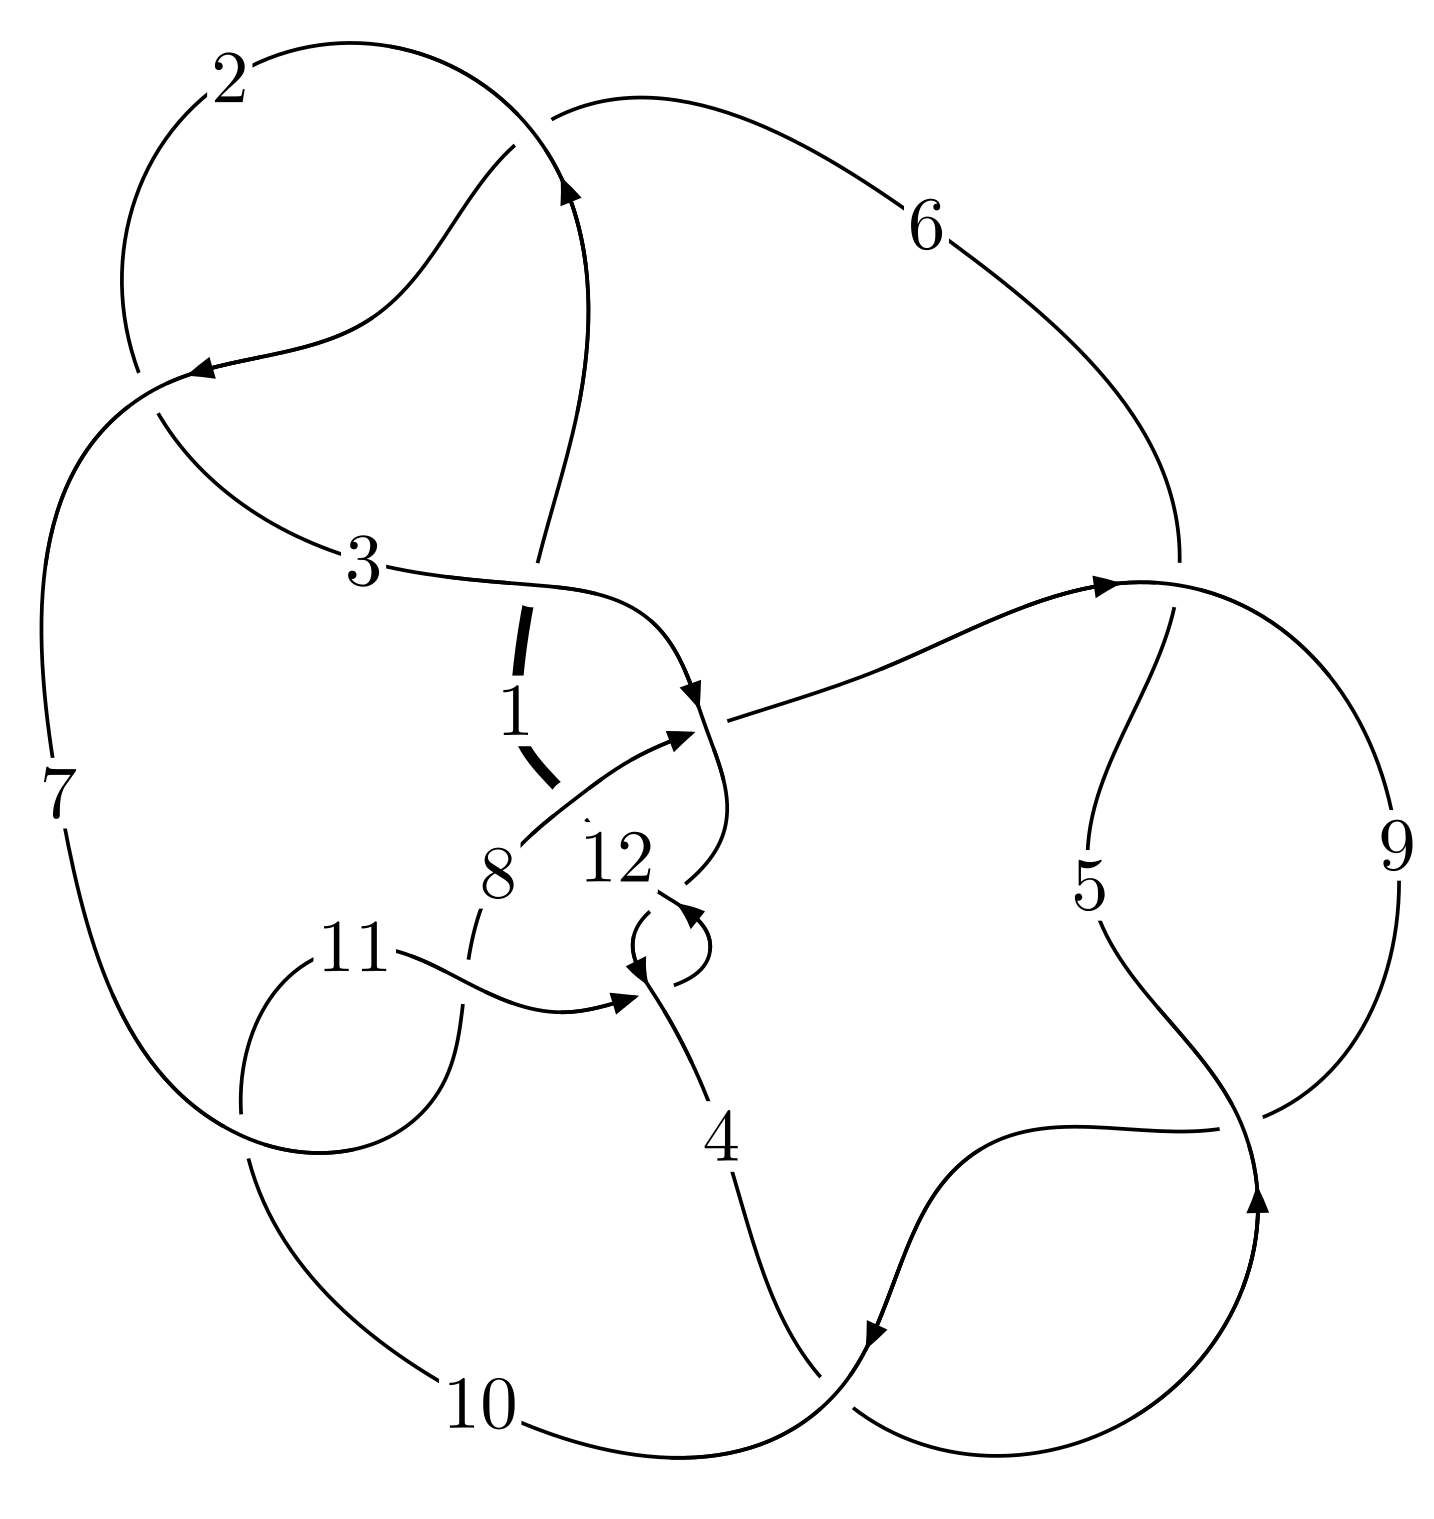
\includegraphics[width=112pt]{../../../GIT/diagram.site/Diagrams/png/2674_12n_0585.png}\\
\ \ \ A knot diagram\footnotemark}&
\allowdisplaybreaks
\textbf{Linearized knot diagam} \\
\cline{2-2}
 &
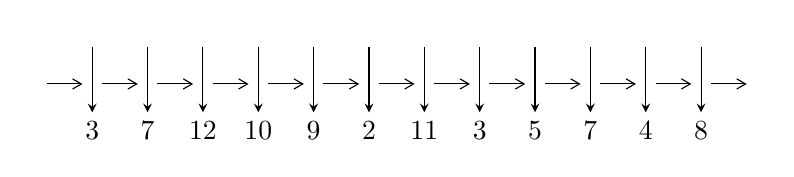
\begin{tikzpicture}[x=20pt, y=17pt]
	% nodes
	\node (C0) at (0, 0) {};
	\node (C1) at (1, 0) {};
	\node (C1U) at (1, +1) {};
	\node (C1D) at (1, -1) {3};

	\node (C2) at (2, 0) {};
	\node (C2U) at (2, +1) {};
	\node (C2D) at (2, -1) {7};

	\node (C3) at (3, 0) {};
	\node (C3U) at (3, +1) {};
	\node (C3D) at (3, -1) {12};

	\node (C4) at (4, 0) {};
	\node (C4U) at (4, +1) {};
	\node (C4D) at (4, -1) {10};

	\node (C5) at (5, 0) {};
	\node (C5U) at (5, +1) {};
	\node (C5D) at (5, -1) {9};

	\node (C6) at (6, 0) {};
	\node (C6U) at (6, +1) {};
	\node (C6D) at (6, -1) {2};

	\node (C7) at (7, 0) {};
	\node (C7U) at (7, +1) {};
	\node (C7D) at (7, -1) {11};

	\node (C8) at (8, 0) {};
	\node (C8U) at (8, +1) {};
	\node (C8D) at (8, -1) {3};

	\node (C9) at (9, 0) {};
	\node (C9U) at (9, +1) {};
	\node (C9D) at (9, -1) {5};

	\node (C10) at (10, 0) {};
	\node (C10U) at (10, +1) {};
	\node (C10D) at (10, -1) {7};

	\node (C11) at (11, 0) {};
	\node (C11U) at (11, +1) {};
	\node (C11D) at (11, -1) {4};

	\node (C12) at (12, 0) {};
	\node (C12U) at (12, +1) {};
	\node (C12D) at (12, -1) {8};
	\node (C13) at (13, 0) {};

	% arrows
	\draw[->,>={angle 60}]
	(C0) edge (C1) (C1) edge (C2) (C2) edge (C3) (C3) edge (C4) (C4) edge (C5) (C5) edge (C6) (C6) edge (C7) (C7) edge (C8) (C8) edge (C9) (C9) edge (C10) (C10) edge (C11) (C11) edge (C12) (C12) edge (C13) ;	\draw[->,>=stealth]
	(C1U) edge (C1D) (C2U) edge (C2D) (C3U) edge (C3D) (C4U) edge (C4D) (C5U) edge (C5D) (C6U) edge (C6D) (C7U) edge (C7D) (C8U) edge (C8D) (C9U) edge (C9D) (C10U) edge (C10D) (C11U) edge (C11D) (C12U) edge (C12D) ;
	\end{tikzpicture} \\
\hhline{~~} \\& 
\textbf{Solving Sequence} \\ \cline{2-2} 
 &
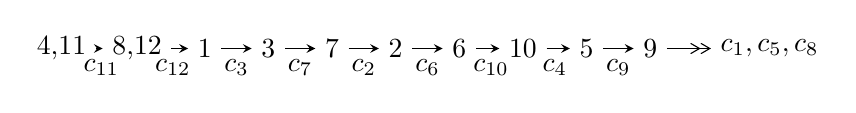
\begin{tikzpicture}[x=23pt, y=7pt]
	% node
	\node (A0) at (-1/8, 0) {4,11};
	\node (A1) at (17/16, 0) {8,12};
	\node (A2) at (17/8, 0) {1};
	\node (A3) at (25/8, 0) {3};
	\node (A4) at (33/8, 0) {7};
	\node (A5) at (41/8, 0) {2};
	\node (A6) at (49/8, 0) {6};
	\node (A7) at (57/8, 0) {10};
	\node (A8) at (65/8, 0) {5};
	\node (A9) at (73/8, 0) {9};
	\node (C1) at (1/2, -1) {$c_{11}$};
	\node (C2) at (13/8, -1) {$c_{12}$};
	\node (C3) at (21/8, -1) {$c_{3}$};
	\node (C4) at (29/8, -1) {$c_{7}$};
	\node (C5) at (37/8, -1) {$c_{2}$};
	\node (C6) at (45/8, -1) {$c_{6}$};
	\node (C7) at (53/8, -1) {$c_{10}$};
	\node (C8) at (61/8, -1) {$c_{4}$};
	\node (C9) at (69/8, -1) {$c_{9}$};
	\node (A10) at (11, 0) {$c_{1},c_{5},c_{8}$};

	% edge
	\draw[->,>=stealth]	
	(A0) edge (A1) (A1) edge (A2) (A2) edge (A3) (A3) edge (A4) (A4) edge (A5) (A5) edge (A6) (A6) edge (A7) (A7) edge (A8) (A8) edge (A9) ;
	\draw[->>,>={angle 60}]	
	(A9) edge (A10);
\end{tikzpicture} \\ 

\end{tabular} \\

\footnotetext{
The image of knot diagram is generated by the software ``\textbf{Draw programme}" developed by Andrew Bartholomew(\url{http://www.layer8.co.uk/maths/draw/index.htm\#Running-draw}), where we modified some parts for our purpose(\url{https://github.com/CATsTAILs/LinksPainter}).
}\phantom \\ \newline 
\centering \textbf{Ideals for irreducible components\footnotemark of $X_{\text{par}}$} 
 
\begin{align*}
I^u_{1}&=\langle 
-3 u^{19}-26 u^{18}+\cdots+2 b+8,\;u^{19}+13 u^{18}+\cdots+2 a-25,\;u^{20}+8 u^{19}+\cdots-10 u-4\rangle \\
I^u_{2}&=\langle 
367 u^4 a^3-289 u^4 a^2+\cdots+163 a-69,\;- u^4 a-9 u^4+\cdots-2 a^3+3 a^2,\;u^5- u^4+2 u^3- u^2+u-1\rangle \\
I^u_{3}&=\langle 
u^{12}-2 u^{11}+8 u^{10}-12 u^9+23 u^8-26 u^7+31 u^6-25 u^5+19 u^4-8 u^3+3 u^2+b+u-1,\\
\phantom{I^u_{3}}&\phantom{= \langle  }-4 u^{12}+12 u^{11}+\cdots+3 a-5,\\
\phantom{I^u_{3}}&\phantom{= \langle  }u^{13}-3 u^{12}+11 u^{11}-22 u^{10}+43 u^9-62 u^8+82 u^7-89 u^6+85 u^5-68 u^4+46 u^3-25 u^2+11 u-3\rangle \\
\\
\end{align*}
\raggedright * 3 irreducible components of $\dim_{\mathbb{C}}=0$, with total 53 representations.\\
\footnotetext{All coefficients of polynomials are rational numbers. But the coefficients are sometimes approximated in decimal forms when there is not enough margin.}
\newpage
\renewcommand{\arraystretch}{1}
\centering \section*{I. $I^u_{1}= \langle -3 u^{19}-26 u^{18}+\cdots+2 b+8,\;u^{19}+13 u^{18}+\cdots+2 a-25,\;u^{20}+8 u^{19}+\cdots-10 u-4 \rangle$}
\flushleft \textbf{(i) Arc colorings}\\
\begin{tabular}{m{7pt} m{180pt} m{7pt} m{180pt} }
\flushright $a_{4}=$&$\begin{pmatrix}0\\u\end{pmatrix}$ \\
\flushright $a_{11}=$&$\begin{pmatrix}1\\0\end{pmatrix}$ \\
\flushright $a_{8}=$&$\begin{pmatrix}-\frac{1}{2} u^{19}-\frac{13}{2} u^{18}+\cdots+\frac{59}{2} u+\frac{25}{2}\\\frac{3}{2} u^{19}+13 u^{18}+\cdots-\frac{37}{2} u-4\end{pmatrix}$ \\
\flushright $a_{12}=$&$\begin{pmatrix}1\\u^2\end{pmatrix}$ \\
\flushright $a_{1}=$&$\begin{pmatrix}\frac{1}{4} u^{19}+\frac{3}{2} u^{18}+\cdots+\frac{3}{4} u+1\\-\frac{1}{2} u^{19}-3 u^{18}+\cdots+\frac{3}{2} u+1\end{pmatrix}$ \\
\flushright $a_{3}=$&$\begin{pmatrix}u\\u^3+u\end{pmatrix}$ \\
\flushright $a_{7}=$&$\begin{pmatrix}u^{19}+\frac{13}{2} u^{18}+\cdots+11 u+\frac{17}{2}\\\frac{3}{2} u^{19}+13 u^{18}+\cdots-\frac{37}{2} u-4\end{pmatrix}$ \\
\flushright $a_{2}=$&$\begin{pmatrix}\frac{1}{4} u^{19}+\frac{3}{2} u^{18}+\cdots-\frac{5}{4} u-1\\\frac{1}{2} u^{19}+3 u^{18}+\cdots-\frac{1}{2} u-1\end{pmatrix}$ \\
\flushright $a_{6}=$&$\begin{pmatrix}\frac{7}{4} u^{19}+\frac{25}{2} u^{18}+\cdots+\frac{9}{4} u+3\\\frac{3}{2} u^{19}+11 u^{18}+\cdots-\frac{43}{2} u-9\end{pmatrix}$ \\
\flushright $a_{10}=$&$\begin{pmatrix}\frac{3}{4} u^{19}+\frac{9}{2} u^{18}+\cdots+\frac{1}{4} u+3\\\frac{3}{2} u^{19}+11 u^{18}+\cdots-\frac{19}{2} u-3\end{pmatrix}$ \\
\flushright $a_{5}=$&$\begin{pmatrix}- u^{19}-\frac{11}{2} u^{18}+\cdots-13 u-\frac{21}{2}\\-\frac{7}{2} u^{19}-27 u^{18}+\cdots+\frac{67}{2} u+10\end{pmatrix}$ \\
\flushright $a_{9}=$&$\begin{pmatrix}\frac{3}{2} u^{19}+\frac{21}{2} u^{18}+\cdots+\frac{9}{2} u+\frac{5}{2}\\\frac{3}{2} u^{19}+12 u^{18}+\cdots-\frac{51}{2} u-10\end{pmatrix}$\\&\end{tabular}
\flushleft \textbf{(ii) Obstruction class $= -1$}\\~\\
\flushleft \textbf{(iii) Cusp Shapes $= 3 u^{19}+21 u^{18}+95 u^{17}+306 u^{16}+777 u^{15}+1606 u^{14}+2750 u^{13}+3938 u^{12}+4673 u^{11}+4519 u^{10}+3361 u^9+1582 u^8-119 u^7-1191 u^6-1413 u^5-1054 u^4-527 u^3-148 u^2-6 u+6$}\\~\\
\newpage\renewcommand{\arraystretch}{1}
\flushleft \textbf{(iv) u-Polynomials at the component}\newline \\
\begin{tabular}{m{50pt}|m{274pt}}
Crossings & \hspace{64pt}u-Polynomials at each crossing \\
\hline $$\begin{aligned}c_{1}\end{aligned}$$&$\begin{aligned}
&u^{20}+29 u^{19}+\cdots+6 u+1
\end{aligned}$\\
\hline $$\begin{aligned}c_{2},c_{6},c_{12}\end{aligned}$$&$\begin{aligned}
&u^{20}- u^{19}+\cdots+3 u^2-1
\end{aligned}$\\
\hline $$\begin{aligned}c_{3},c_{11}\end{aligned}$$&$\begin{aligned}
&u^{20}-8 u^{19}+\cdots+10 u-4
\end{aligned}$\\
\hline $$\begin{aligned}c_{4},c_{5},c_{9}\end{aligned}$$&$\begin{aligned}
&u^{20}+11 u^{19}+\cdots+352 u+32
\end{aligned}$\\
\hline $$\begin{aligned}c_{7},c_{10}\end{aligned}$$&$\begin{aligned}
&u^{20}+u^{19}+\cdots- u-1
\end{aligned}$\\
\hline $$\begin{aligned}c_{8}\end{aligned}$$&$\begin{aligned}
&u^{20}-20 u^{18}+\cdots+363 u+389
\end{aligned}$\\
\hline
\end{tabular}\\~\\
\newpage\renewcommand{\arraystretch}{1}
\flushleft \textbf{(v) Riley Polynomials at the component}\newline \\
\begin{tabular}{m{50pt}|m{274pt}}
Crossings & \hspace{64pt}Riley Polynomials at each crossing \\
\hline $$\begin{aligned}c_{1}\end{aligned}$$&$\begin{aligned}
&y^{20}-77 y^{19}+\cdots-30 y+1
\end{aligned}$\\
\hline $$\begin{aligned}c_{2},c_{6},c_{12}\end{aligned}$$&$\begin{aligned}
&y^{20}-29 y^{19}+\cdots-6 y+1
\end{aligned}$\\
\hline $$\begin{aligned}c_{3},c_{11}\end{aligned}$$&$\begin{aligned}
&y^{20}+16 y^{19}+\cdots-124 y+16
\end{aligned}$\\
\hline $$\begin{aligned}c_{4},c_{5},c_{9}\end{aligned}$$&$\begin{aligned}
&y^{20}+17 y^{19}+\cdots-8704 y+1024
\end{aligned}$\\
\hline $$\begin{aligned}c_{7},c_{10}\end{aligned}$$&$\begin{aligned}
&y^{20}-19 y^{19}+\cdots-11 y+1
\end{aligned}$\\
\hline $$\begin{aligned}c_{8}\end{aligned}$$&$\begin{aligned}
&y^{20}-40 y^{19}+\cdots-327047 y+151321
\end{aligned}$\\
\hline
\end{tabular}\\~\\
\newpage\flushleft \textbf{(vi) Complex Volumes and Cusp Shapes}
$$\begin{array}{c|c|c}  
\text{Solutions to }I^u_{1}& \I (\text{vol} + \sqrt{-1}CS) & \text{Cusp shape}\\
 \hline 
\begin{aligned}
u &= -0.307939 + 0.948375 I \\
a &= \phantom{-}0.05622 + 1.79329 I \\
b &= \phantom{-}1.20587 - 0.93158 I\end{aligned}
 & \phantom{-}3.89445 + 4.62827 I & -7.73780 - 0.37198 I \\ \hline\begin{aligned}
u &= -0.307939 - 0.948375 I \\
a &= \phantom{-}0.05622 - 1.79329 I \\
b &= \phantom{-}1.20587 + 0.93158 I\end{aligned}
 & \phantom{-}3.89445 - 4.62827 I & -7.73780 + 0.37198 I \\ \hline\begin{aligned}
u &= \phantom{-}0.186964 + 0.988512 I \\
a &= -0.089455 + 0.771960 I \\
b &= \phantom{-}0.364770 - 0.350879 I\end{aligned}
 & \phantom{-}1.95473 - 1.84370 I & -7.61677 + 4.71510 I \\ \hline\begin{aligned}
u &= \phantom{-}0.186964 - 0.988512 I \\
a &= -0.089455 - 0.771960 I \\
b &= \phantom{-}0.364770 + 0.350879 I\end{aligned}
 & \phantom{-}1.95473 + 1.84370 I & -7.61677 - 4.71510 I \\ \hline\begin{aligned}
u &= -0.219887 + 0.859832 I \\
a &= \phantom{-}0.26086 - 1.47452 I \\
b &= -1.050500 + 0.454707 I\end{aligned}
 & -0.445235 + 1.140740 I & -12.74589 - 1.01888 I \\ \hline\begin{aligned}
u &= -0.219887 - 0.859832 I \\
a &= \phantom{-}0.26086 + 1.47452 I \\
b &= -1.050500 - 0.454707 I\end{aligned}
 & -0.445235 - 1.140740 I & -12.74589 + 1.01888 I \\ \hline\begin{aligned}
u &= -1.165370 + 0.101289 I \\
a &= \phantom{-}0.249791 - 0.036181 I \\
b &= -1.44567 - 0.47752 I\end{aligned}
 & -10.71860 - 7.16687 I & -14.7672 + 3.4591 I \\ \hline\begin{aligned}
u &= -1.165370 - 0.101289 I \\
a &= \phantom{-}0.249791 + 0.036181 I \\
b &= -1.44567 + 0.47752 I\end{aligned}
 & -10.71860 + 7.16687 I & -14.7672 - 3.4591 I \\ \hline\begin{aligned}
u &= -1.17535\phantom{ +0.000000I} \\
a &= -0.236789\phantom{ +0.000000I} \\
b &= \phantom{-}1.58721\phantom{ +0.000000I}\end{aligned}
 & -15.2605\phantom{ +0.000000I} & -16.9350\phantom{ +0.000000I} \\ \hline\begin{aligned}
u &= -0.319592 + 0.523784 I \\
a &= -0.734866 + 1.076110 I \\
b &= \phantom{-}0.821178 + 0.439010 I\end{aligned}
 & \phantom{-}2.81143 - 1.78462 I & -5.22189 + 4.40876 I\\
 \hline 
 \end{array}$$\newpage$$\begin{array}{c|c|c}  
\text{Solutions to }I^u_{1}& \I (\text{vol} + \sqrt{-1}CS) & \text{Cusp shape}\\
 \hline 
\begin{aligned}
u &= -0.319592 - 0.523784 I \\
a &= -0.734866 - 1.076110 I \\
b &= \phantom{-}0.821178 - 0.439010 I\end{aligned}
 & \phantom{-}2.81143 + 1.78462 I & -5.22189 - 4.40876 I \\ \hline\begin{aligned}
u &= -0.62192 + 1.33439 I \\
a &= \phantom{-}0.48413 - 1.57383 I \\
b &= -1.48076 + 0.92864 I\end{aligned}
 & -6.9069 + 13.4360 I & -11.74255 - 6.57313 I \\ \hline\begin{aligned}
u &= -0.62192 - 1.33439 I \\
a &= \phantom{-}0.48413 + 1.57383 I \\
b &= -1.48076 - 0.92864 I\end{aligned}
 & -6.9069 - 13.4360 I & -11.74255 + 6.57313 I \\ \hline\begin{aligned}
u &= -0.61063 + 1.39810 I \\
a &= -0.81610 + 1.20565 I \\
b &= \phantom{-}1.46551 - 0.44107 I\end{aligned}
 & -10.94070 + 6.30161 I & -14.3965 - 3.2767 I \\ \hline\begin{aligned}
u &= -0.61063 - 1.39810 I \\
a &= -0.81610 - 1.20565 I \\
b &= \phantom{-}1.46551 + 0.44107 I\end{aligned}
 & -10.94070 - 6.30161 I & -14.3965 + 3.2767 I \\ \hline\begin{aligned}
u &= \phantom{-}0.09565 + 1.60341 I \\
a &= -0.332044 - 0.380939 I \\
b &= \phantom{-}0.073621 + 0.411439 I\end{aligned}
 & \phantom{-}10.12870 - 1.84544 I & -0.92402 + 4.93320 I \\ \hline\begin{aligned}
u &= \phantom{-}0.09565 - 1.60341 I \\
a &= -0.332044 + 0.380939 I \\
b &= \phantom{-}0.073621 - 0.411439 I\end{aligned}
 & \phantom{-}10.12870 + 1.84544 I & -0.92402 - 4.93320 I \\ \hline\begin{aligned}
u &= -0.57369 + 1.50037 I \\
a &= \phantom{-}0.895185 - 0.618003 I \\
b &= -1.119450 - 0.042363 I\end{aligned}
 & -5.72650 - 0.92873 I & -13.76270 + 0.38685 I \\ \hline\begin{aligned}
u &= -0.57369 - 1.50037 I \\
a &= \phantom{-}0.895185 + 0.618003 I \\
b &= -1.119450 + 0.042363 I\end{aligned}
 & -5.72650 + 0.92873 I & -13.76270 - 0.38685 I \\ \hline\begin{aligned}
u &= \phantom{-}0.248179\phantom{ +0.000000I} \\
a &= \phantom{-}1.28936\phantom{ +0.000000I} \\
b &= -0.256367\phantom{ +0.000000I}\end{aligned}
 & -0.545579\phantom{ +0.000000I} & -18.2350\phantom{ +0.000000I}\\
 \hline 
 \end{array}$$\newpage\newpage\renewcommand{\arraystretch}{1}
\centering \section*{II. $I^u_{2}= \langle 367 u^4 a^3-289 u^4 a^2+\cdots+163 a-69,\;- u^4 a-9 u^4+\cdots-2 a^3+3 a^2,\;u^5- u^4+2 u^3- u^2+u-1 \rangle$}
\flushleft \textbf{(i) Arc colorings}\\
\begin{tabular}{m{7pt} m{180pt} m{7pt} m{180pt} }
\flushright $a_{4}=$&$\begin{pmatrix}0\\u\end{pmatrix}$ \\
\flushright $a_{11}=$&$\begin{pmatrix}1\\0\end{pmatrix}$ \\
\flushright $a_{8}=$&$\begin{pmatrix}a\\-1.80788 a^{3} u^{4}+1.42365 a^{2} u^{4}+\cdots-0.802956 a+0.339901\end{pmatrix}$ \\
\flushright $a_{12}=$&$\begin{pmatrix}1\\u^2\end{pmatrix}$ \\
\flushright $a_{1}=$&$\begin{pmatrix}-0.817734 a^{3} u^{4}+1.02463 a^{2} u^{4}+\cdots-0.556650 a+2.72906\\-\frac{8}{7} u^4 a^2-\frac{4}{7} u^4+\cdots-\frac{6}{7} a^2+\frac{4}{7}\end{pmatrix}$ \\
\flushright $a_{3}=$&$\begin{pmatrix}u\\u^3+u\end{pmatrix}$ \\
\flushright $a_{7}=$&$\begin{pmatrix}-1.80788 a^{3} u^{4}+1.42365 a^{2} u^{4}+\cdots+0.197044 a+0.339901\\-1.80788 a^{3} u^{4}+1.42365 a^{2} u^{4}+\cdots-0.802956 a+0.339901\end{pmatrix}$ \\
\flushright $a_{2}=$&$\begin{pmatrix}-1.31527 a^{3} u^{4}+1.80296 a^{2} u^{4}+\cdots-1.11823 a+2.16749\\-1.20197 a^{3} u^{4}+1.03448 a^{2} u^{4}+\cdots-0.950739 a+0.620690\end{pmatrix}$ \\
\flushright $a_{6}=$&$\begin{pmatrix}-0.945813 a^{3} u^{4}+0.837438 a^{2} u^{4}+\cdots-1.35468 a-1.21182\\0.359606 a^{3} u^{4}+0.492611 a^{2} u^{4}+\cdots+0.00985222 a+0.581281\end{pmatrix}$ \\
\flushright $a_{10}=$&$\begin{pmatrix}0.945813 a^{3} u^{4}-0.837438 a^{2} u^{4}+\cdots+1.35468 a-0.788177\\0.128079 a^{3} u^{4}+0.187192 a^{2} u^{4}+\cdots+0.798030 a-0.0591133\end{pmatrix}$ \\
\flushright $a_{5}=$&$\begin{pmatrix}0.945813 a^{3} u^{4}-0.837438 a^{2} u^{4}+\cdots+1.35468 a+0.211823\\0.133005 a^{3} u^{4}-0.399015 a^{2} u^{4}+\cdots+0.674877 a-0.610837\end{pmatrix}$ \\
\flushright $a_{9}=$&$\begin{pmatrix}0.945813 a^{3} u^{4}-0.837438 a^{2} u^{4}+\cdots+1.35468 a+0.211823\\-0.364532 a^{3} u^{4}+0.0935961 a^{2} u^{4}+\cdots+0.113300 a-0.0295567\end{pmatrix}$\\&\end{tabular}
\flushleft \textbf{(ii) Obstruction class $= -1$}\\~\\
\flushleft \textbf{(iii) Cusp Shapes $= -\frac{492}{203} u^4 a^3+\frac{664}{203} u^4 a^2+\cdots-\frac{692}{203} a-\frac{2026}{203}$}\\~\\
\newpage\renewcommand{\arraystretch}{1}
\flushleft \textbf{(iv) u-Polynomials at the component}\newline \\
\begin{tabular}{m{50pt}|m{274pt}}
Crossings & \hspace{64pt}u-Polynomials at each crossing \\
\hline $$\begin{aligned}c_{1}\end{aligned}$$&$\begin{aligned}
&u^{20}+25 u^{19}+\cdots+3332 u+10609
\end{aligned}$\\
\hline $$\begin{aligned}c_{2},c_{6},c_{12}\end{aligned}$$&$\begin{aligned}
&u^{20}- u^{19}+\cdots+6 u+103
\end{aligned}$\\
\hline $$\begin{aligned}c_{3},c_{11}\end{aligned}$$&$\begin{aligned}
&(u^5+u^4+2 u^3+u^2+u+1)^4
\end{aligned}$\\
\hline $$\begin{aligned}c_{4},c_{5},c_{9}\end{aligned}$$&$\begin{aligned}
&(u^2- u+1)^{10}
\end{aligned}$\\
\hline $$\begin{aligned}c_{7},c_{10}\end{aligned}$$&$\begin{aligned}
&u^{20}+5 u^{19}+\cdots-8 u+1
\end{aligned}$\\
\hline $$\begin{aligned}c_{8}\end{aligned}$$&$\begin{aligned}
&u^{20}+u^{19}+\cdots+1242 u+1549
\end{aligned}$\\
\hline
\end{tabular}\\~\\
\newpage\renewcommand{\arraystretch}{1}
\flushleft \textbf{(v) Riley Polynomials at the component}\newline \\
\begin{tabular}{m{50pt}|m{274pt}}
Crossings & \hspace{64pt}Riley Polynomials at each crossing \\
\hline $$\begin{aligned}c_{1}\end{aligned}$$&$\begin{aligned}
&y^{20}-53 y^{19}+\cdots+3723477956 y+112550881
\end{aligned}$\\
\hline $$\begin{aligned}c_{2},c_{6},c_{12}\end{aligned}$$&$\begin{aligned}
&y^{20}-25 y^{19}+\cdots-3332 y+10609
\end{aligned}$\\
\hline $$\begin{aligned}c_{3},c_{11}\end{aligned}$$&$\begin{aligned}
&(y^5+3 y^4+4 y^3+y^2- y-1)^4
\end{aligned}$\\
\hline $$\begin{aligned}c_{4},c_{5},c_{9}\end{aligned}$$&$\begin{aligned}
&(y^2+y+1)^{10}
\end{aligned}$\\
\hline $$\begin{aligned}c_{7},c_{10}\end{aligned}$$&$\begin{aligned}
&y^{20}-5 y^{19}+\cdots+212 y+1
\end{aligned}$\\
\hline $$\begin{aligned}c_{8}\end{aligned}$$&$\begin{aligned}
&y^{20}-33 y^{19}+\cdots-1381468 y+2399401
\end{aligned}$\\
\hline
\end{tabular}\\~\\
\newpage\flushleft \textbf{(vi) Complex Volumes and Cusp Shapes}
$$\begin{array}{c|c|c}  
\text{Solutions to }I^u_{2}& \I (\text{vol} + \sqrt{-1}CS) & \text{Cusp shape}\\
 \hline 
\begin{aligned}
u &= -0.339110 + 0.822375 I \\
a &= -1.24082 + 0.82885 I \\
b &= -0.839233 + 0.066856 I\end{aligned}
 & -4.60570 - 0.49930 I & -15.4849 - 0.9665 I \\ \hline\begin{aligned}
u &= -0.339110 + 0.822375 I \\
a &= \phantom{-}1.51588 + 1.67630 I \\
b &= -1.43083 - 1.67189 I\end{aligned}
 & -4.60570 + 3.56046 I & -15.4849 - 7.8947 I \\ \hline\begin{aligned}
u &= -0.339110 + 0.822375 I \\
a &= \phantom{-}1.09190 - 2.13507 I \\
b &= \phantom{-}0.0324686 - 0.0684453 I\end{aligned}
 & -4.60570 + 3.56046 I & -15.4849 - 7.8947 I \\ \hline\begin{aligned}
u &= -0.339110 + 0.822375 I \\
a &= -0.46038 - 2.85787 I \\
b &= \phantom{-}0.03124 + 2.01433 I\end{aligned}
 & -4.60570 - 0.49930 I & -15.4849 - 0.9665 I \\ \hline\begin{aligned}
u &= -0.339110 - 0.822375 I \\
a &= -1.24082 - 0.82885 I \\
b &= -0.839233 - 0.066856 I\end{aligned}
 & -4.60570 + 0.49930 I & -15.4849 + 0.9665 I \\ \hline\begin{aligned}
u &= -0.339110 - 0.822375 I \\
a &= \phantom{-}1.51588 - 1.67630 I \\
b &= -1.43083 + 1.67189 I\end{aligned}
 & -4.60570 - 3.56046 I & -15.4849 + 7.8947 I \\ \hline\begin{aligned}
u &= -0.339110 - 0.822375 I \\
a &= \phantom{-}1.09190 + 2.13507 I \\
b &= \phantom{-}0.0324686 + 0.0684453 I\end{aligned}
 & -4.60570 - 3.56046 I & -15.4849 + 7.8947 I \\ \hline\begin{aligned}
u &= -0.339110 - 0.822375 I \\
a &= -0.46038 + 2.85787 I \\
b &= \phantom{-}0.03124 - 2.01433 I\end{aligned}
 & -4.60570 + 0.49930 I & -15.4849 + 0.9665 I \\ \hline\begin{aligned}
u &= \phantom{-}0.766826\phantom{ +0.000000I} \\
a &= \phantom{-}0.651697 + 0.410335 I \\
b &= \phantom{-}1.034330 - 0.571171 I\end{aligned}
 & -2.53372 + 2.02988 I & -14.5189 - 3.4641 I \\ \hline\begin{aligned}
u &= \phantom{-}0.766826\phantom{ +0.000000I} \\
a &= \phantom{-}0.651697 - 0.410335 I \\
b &= \phantom{-}1.034330 + 0.571171 I\end{aligned}
 & -2.53372 - 2.02988 I & -14.5189 + 3.4641 I\\
 \hline 
 \end{array}$$\newpage$$\begin{array}{c|c|c}  
\text{Solutions to }I^u_{2}& \I (\text{vol} + \sqrt{-1}CS) & \text{Cusp shape}\\
 \hline 
\begin{aligned}
u &= \phantom{-}0.766826\phantom{ +0.000000I} \\
a &= -0.055956 + 0.621518 I \\
b &= -1.292890 + 0.123332 I\end{aligned}
 & -2.53372 + 2.02988 I & -14.5189 - 3.4641 I \\ \hline\begin{aligned}
u &= \phantom{-}0.766826\phantom{ +0.000000I} \\
a &= -0.055956 - 0.621518 I \\
b &= -1.292890 - 0.123332 I\end{aligned}
 & -2.53372 - 2.02988 I & -14.5189 + 3.4641 I \\ \hline\begin{aligned}
u &= \phantom{-}0.455697 + 1.200150 I \\
a &= -0.846255 - 0.412340 I \\
b &= \phantom{-}1.265170 - 0.048633 I\end{aligned}
 & \phantom{-}0.93776 - 2.37095 I & -11.25569 + 0.03448 I \\ \hline\begin{aligned}
u &= \phantom{-}0.455697 + 1.200150 I \\
a &= \phantom{-}0.429720 + 1.227490 I \\
b &= -0.744138 - 0.292701 I\end{aligned}
 & \phantom{-}0.93776 - 2.37095 I & -11.25569 + 0.03448 I \\ \hline\begin{aligned}
u &= \phantom{-}0.455697 + 1.200150 I \\
a &= \phantom{-}0.11602 - 1.56704 I \\
b &= \phantom{-}1.022890 + 0.683808 I\end{aligned}
 & \phantom{-}0.93776 - 6.43072 I & -11.25569 + 6.96269 I \\ \hline\begin{aligned}
u &= \phantom{-}0.455697 + 1.200150 I \\
a &= \phantom{-}0.79819 + 1.52019 I \\
b &= -1.57901 - 0.96437 I\end{aligned}
 & \phantom{-}0.93776 - 6.43072 I & -11.25569 + 6.96269 I \\ \hline\begin{aligned}
u &= \phantom{-}0.455697 - 1.200150 I \\
a &= -0.846255 + 0.412340 I \\
b &= \phantom{-}1.265170 + 0.048633 I\end{aligned}
 & \phantom{-}0.93776 + 2.37095 I & -11.25569 - 0.03448 I \\ \hline\begin{aligned}
u &= \phantom{-}0.455697 - 1.200150 I \\
a &= \phantom{-}0.429720 - 1.227490 I \\
b &= -0.744138 + 0.292701 I\end{aligned}
 & \phantom{-}0.93776 + 2.37095 I & -11.25569 - 0.03448 I \\ \hline\begin{aligned}
u &= \phantom{-}0.455697 - 1.200150 I \\
a &= \phantom{-}0.11602 + 1.56704 I \\
b &= \phantom{-}1.022890 - 0.683808 I\end{aligned}
 & \phantom{-}0.93776 + 6.43072 I & -11.25569 - 6.96269 I \\ \hline\begin{aligned}
u &= \phantom{-}0.455697 - 1.200150 I \\
a &= \phantom{-}0.79819 - 1.52019 I \\
b &= -1.57901 + 0.96437 I\end{aligned}
 & \phantom{-}0.93776 + 6.43072 I & -11.25569 - 6.96269 I\\
 \hline 
 \end{array}$$\newpage\newpage\renewcommand{\arraystretch}{1}
\centering \section*{III. $I^u_{3}= \langle u^{12}-2 u^{11}+\cdots+b-1,\;-4 u^{12}+12 u^{11}+\cdots+3 a-5,\;u^{13}-3 u^{12}+\cdots+11 u-3 \rangle$}
\flushleft \textbf{(i) Arc colorings}\\
\begin{tabular}{m{7pt} m{180pt} m{7pt} m{180pt} }
\flushright $a_{4}=$&$\begin{pmatrix}0\\u\end{pmatrix}$ \\
\flushright $a_{11}=$&$\begin{pmatrix}1\\0\end{pmatrix}$ \\
\flushright $a_{8}=$&$\begin{pmatrix}\frac{4}{3} u^{12}-4 u^{11}+\cdots-\frac{31}{3} u+\frac{5}{3}\\- u^{12}+2 u^{11}+\cdots- u+1\end{pmatrix}$ \\
\flushright $a_{12}=$&$\begin{pmatrix}1\\u^2\end{pmatrix}$ \\
\flushright $a_{1}=$&$\begin{pmatrix}-\frac{2}{3} u^{12}+3 u^{11}+\cdots+\frac{14}{3} u+\frac{2}{3}\\u^{12}-3 u^{11}+\cdots-3 u+1\end{pmatrix}$ \\
\flushright $a_{3}=$&$\begin{pmatrix}u\\u^3+u\end{pmatrix}$ \\
\flushright $a_{7}=$&$\begin{pmatrix}\frac{1}{3} u^{12}-2 u^{11}+\cdots-\frac{34}{3} u+\frac{8}{3}\\- u^{12}+2 u^{11}+\cdots- u+1\end{pmatrix}$ \\
\flushright $a_{2}=$&$\begin{pmatrix}\frac{1}{3} u^{12}+\frac{2}{3} u^{10}+\cdots+\frac{8}{3} u+\frac{2}{3}\\u^{12}-3 u^{11}+\cdots-2 u+1\end{pmatrix}$ \\
\flushright $a_{6}=$&$\begin{pmatrix}- u^3+u^2-2 u+1\\u^{12}-3 u^{11}+\cdots-15 u^3+4 u^2\end{pmatrix}$ \\
\flushright $a_{10}=$&$\begin{pmatrix}-\frac{1}{3} u^{12}+u^{11}+\cdots+\frac{4}{3} u-\frac{2}{3}\\- u^{10}+2 u^9+\cdots+2 u-1\end{pmatrix}$ \\
\flushright $a_{5}=$&$\begin{pmatrix}\frac{2}{3} u^{12}-2 u^{11}+\cdots-\frac{17}{3} u+\frac{7}{3}\\-2 u^{11}+4 u^{10}+\cdots-5 u+2\end{pmatrix}$ \\
\flushright $a_{9}=$&$\begin{pmatrix}\frac{1}{3} u^{12}- u^{11}+\cdots-\frac{19}{3} u+\frac{5}{3}\\- u^{12}+3 u^{11}+\cdots-6 u^2+1\end{pmatrix}$\\&\end{tabular}
\flushleft \textbf{(ii) Obstruction class $= 1$}\\~\\
\flushleft \textbf{(iii) Cusp Shapes $= -3 u^{12}+10 u^{11}-33 u^{10}+69 u^9-123 u^8+178 u^7-216 u^6+227 u^5-200 u^4+145 u^3-88 u^2+40 u-24$}\\~\\
\newpage\renewcommand{\arraystretch}{1}
\flushleft \textbf{(iv) u-Polynomials at the component}\newline \\
\begin{tabular}{m{50pt}|m{274pt}}
Crossings & \hspace{64pt}u-Polynomials at each crossing \\
\hline $$\begin{aligned}c_{1}\end{aligned}$$&$\begin{aligned}
&u^{13}-13 u^{12}+\cdots+8 u-1
\end{aligned}$\\
\hline $$\begin{aligned}c_{2}\end{aligned}$$&$\begin{aligned}
&u^{13}- u^{12}+\cdots+4 u^2-1
\end{aligned}$\\
\hline $$\begin{aligned}c_{3}\end{aligned}$$&$\begin{aligned}
&u^{13}+3 u^{12}+\cdots+11 u+3
\end{aligned}$\\
\hline $$\begin{aligned}c_{4},c_{5}\end{aligned}$$&$\begin{aligned}
&u^{13}+8 u^{11}+\cdots+5 u-1
\end{aligned}$\\
\hline $$\begin{aligned}c_{6},c_{12}\end{aligned}$$&$\begin{aligned}
&u^{13}+u^{12}+\cdots-4 u^2+1
\end{aligned}$\\
\hline $$\begin{aligned}c_{7}\end{aligned}$$&$\begin{aligned}
&u^{13}+u^{12}- u^{11}- u^{10}+4 u^9-5 u^7+2 u^5+4 u^3-3 u-1
\end{aligned}$\\
\hline $$\begin{aligned}c_{8}\end{aligned}$$&$\begin{aligned}
&u^{13}-6 u^{11}+\cdots+3 u-1
\end{aligned}$\\
\hline $$\begin{aligned}c_{9}\end{aligned}$$&$\begin{aligned}
&u^{13}+8 u^{11}+\cdots+5 u+1
\end{aligned}$\\
\hline $$\begin{aligned}c_{10}\end{aligned}$$&$\begin{aligned}
&u^{13}- u^{12}- u^{11}+u^{10}+4 u^9-5 u^7+2 u^5+4 u^3-3 u+1
\end{aligned}$\\
\hline $$\begin{aligned}c_{11}\end{aligned}$$&$\begin{aligned}
&u^{13}-3 u^{12}+\cdots+11 u-3
\end{aligned}$\\
\hline
\end{tabular}\\~\\
\newpage\renewcommand{\arraystretch}{1}
\flushleft \textbf{(v) Riley Polynomials at the component}\newline \\
\begin{tabular}{m{50pt}|m{274pt}}
Crossings & \hspace{64pt}Riley Polynomials at each crossing \\
\hline $$\begin{aligned}c_{1}\end{aligned}$$&$\begin{aligned}
&y^{13}-21 y^{12}+\cdots+4 y-1
\end{aligned}$\\
\hline $$\begin{aligned}c_{2},c_{6},c_{12}\end{aligned}$$&$\begin{aligned}
&y^{13}-13 y^{12}+\cdots+8 y-1
\end{aligned}$\\
\hline $$\begin{aligned}c_{3},c_{11}\end{aligned}$$&$\begin{aligned}
&y^{13}+13 y^{12}+\cdots-29 y-9
\end{aligned}$\\
\hline $$\begin{aligned}c_{4},c_{5},c_{9}\end{aligned}$$&$\begin{aligned}
&y^{13}+16 y^{12}+\cdots+11 y-1
\end{aligned}$\\
\hline $$\begin{aligned}c_{7},c_{10}\end{aligned}$$&$\begin{aligned}
&y^{13}-3 y^{12}+\cdots+9 y-1
\end{aligned}$\\
\hline $$\begin{aligned}c_{8}\end{aligned}$$&$\begin{aligned}
&y^{13}-12 y^{12}+\cdots+41 y-1
\end{aligned}$\\
\hline
\end{tabular}\\~\\
\newpage\flushleft \textbf{(vi) Complex Volumes and Cusp Shapes}
$$\begin{array}{c|c|c}  
\text{Solutions to }I^u_{3}& \I (\text{vol} + \sqrt{-1}CS) & \text{Cusp shape}\\
 \hline 
\begin{aligned}
u &= -0.311964 + 1.093350 I \\
a &= \phantom{-}0.774593 - 1.109310 I \\
b &= -0.010328 + 0.900690 I\end{aligned}
 & -2.95271 - 0.68897 I & -9.08547 + 0.28804 I \\ \hline\begin{aligned}
u &= -0.311964 - 1.093350 I \\
a &= \phantom{-}0.774593 + 1.109310 I \\
b &= -0.010328 - 0.900690 I\end{aligned}
 & -2.95271 + 0.68897 I & -9.08547 - 0.28804 I \\ \hline\begin{aligned}
u &= -0.183411 + 0.836579 I \\
a &= -0.25418 + 2.22881 I \\
b &= -0.776793 - 1.074250 I\end{aligned}
 & -4.00352 + 2.67216 I & -9.27660 - 0.66182 I \\ \hline\begin{aligned}
u &= -0.183411 - 0.836579 I \\
a &= -0.25418 - 2.22881 I \\
b &= -0.776793 + 1.074250 I\end{aligned}
 & -4.00352 - 2.67216 I & -9.27660 + 0.66182 I \\ \hline\begin{aligned}
u &= \phantom{-}0.693444 + 0.482308 I \\
a &= -0.323041 - 0.669219 I \\
b &= \phantom{-}1.008100 - 0.435989 I\end{aligned}
 & \phantom{-}1.92069 + 1.38967 I & -14.4640 - 0.3073 I \\ \hline\begin{aligned}
u &= \phantom{-}0.693444 - 0.482308 I \\
a &= -0.323041 + 0.669219 I \\
b &= \phantom{-}1.008100 + 0.435989 I\end{aligned}
 & \phantom{-}1.92069 - 1.38967 I & -14.4640 + 0.3073 I \\ \hline\begin{aligned}
u &= \phantom{-}0.444029 + 1.081590 I \\
a &= -0.07761 - 1.60889 I \\
b &= \phantom{-}1.22506 + 0.94731 I\end{aligned}
 & \phantom{-}3.77211 - 5.65024 I & -8.73340 + 7.27407 I \\ \hline\begin{aligned}
u &= \phantom{-}0.444029 - 1.081590 I \\
a &= -0.07761 + 1.60889 I \\
b &= \phantom{-}1.22506 - 0.94731 I\end{aligned}
 & \phantom{-}3.77211 + 5.65024 I & -8.73340 - 7.27407 I \\ \hline\begin{aligned}
u &= \phantom{-}0.381547 + 1.261190 I \\
a &= \phantom{-}0.456024 + 1.005740 I \\
b &= -0.955954 - 0.399007 I\end{aligned}
 & \phantom{-}1.15315 - 3.75548 I & -9.16700 + 5.96823 I \\ \hline\begin{aligned}
u &= \phantom{-}0.381547 - 1.261190 I \\
a &= \phantom{-}0.456024 - 1.005740 I \\
b &= -0.955954 + 0.399007 I\end{aligned}
 & \phantom{-}1.15315 + 3.75548 I & -9.16700 - 5.96823 I\\
 \hline 
 \end{array}$$\newpage$$\begin{array}{c|c|c}  
\text{Solutions to }I^u_{3}& \I (\text{vol} + \sqrt{-1}CS) & \text{Cusp shape}\\
 \hline 
\begin{aligned}
u &= \phantom{-}0.660856\phantom{ +0.000000I} \\
a &= -0.486065\phantom{ +0.000000I} \\
b &= -0.947145\phantom{ +0.000000I}\end{aligned}
 & -2.65768\phantom{ +0.000000I} & -15.1330\phantom{ +0.000000I} \\ \hline\begin{aligned}
u &= \phantom{-}0.14593 + 1.67508 I \\
a &= -0.499419 - 0.221002 I \\
b &= \phantom{-}0.483481 - 0.069018 I\end{aligned}
 & \phantom{-}9.66379 - 1.70084 I & -17.2072 - 0.2320 I \\ \hline\begin{aligned}
u &= \phantom{-}0.14593 - 1.67508 I \\
a &= -0.499419 + 0.221002 I \\
b &= \phantom{-}0.483481 + 0.069018 I\end{aligned}
 & \phantom{-}9.66379 + 1.70084 I & -17.2072 + 0.2320 I\\
 \hline 
 \end{array}$$\newpage
\newpage\renewcommand{\arraystretch}{1}
\centering \section*{ IV. u-Polynomials}
\begin{tabular}{m{50pt}|m{274pt}}
Crossings & \hspace{64pt}u-Polynomials at each crossing \\
\hline $$\begin{aligned}c_{1}\end{aligned}$$&$\begin{aligned}
&(u^{13}-13 u^{12}+\cdots+8 u-1)(u^{20}+25 u^{19}+\cdots+3332 u+10609)\\
&\cdot(u^{20}+29 u^{19}+\cdots+6 u+1)
\end{aligned}$\\
\hline $$\begin{aligned}c_{2}\end{aligned}$$&$\begin{aligned}
&(u^{13}- u^{12}+\cdots+4 u^2-1)(u^{20}- u^{19}+\cdots+3 u^2-1)\\
&\cdot(u^{20}- u^{19}+\cdots+6 u+103)
\end{aligned}$\\
\hline $$\begin{aligned}c_{3}\end{aligned}$$&$\begin{aligned}
&((u^5+u^4+2 u^3+u^2+u+1)^4)(u^{13}+3 u^{12}+\cdots+11 u+3)\\
&\cdot(u^{20}-8 u^{19}+\cdots+10 u-4)
\end{aligned}$\\
\hline $$\begin{aligned}c_{4},c_{5}\end{aligned}$$&$\begin{aligned}
&((u^2- u+1)^{10})(u^{13}+8 u^{11}+\cdots+5 u-1)\\
&\cdot(u^{20}+11 u^{19}+\cdots+352 u+32)
\end{aligned}$\\
\hline $$\begin{aligned}c_{6},c_{12}\end{aligned}$$&$\begin{aligned}
&(u^{13}+u^{12}+\cdots-4 u^2+1)(u^{20}- u^{19}+\cdots+3 u^2-1)\\
&\cdot(u^{20}- u^{19}+\cdots+6 u+103)
\end{aligned}$\\
\hline $$\begin{aligned}c_{7}\end{aligned}$$&$\begin{aligned}
&(u^{13}+u^{12}- u^{11}- u^{10}+4 u^9-5 u^7+2 u^5+4 u^3-3 u-1)\\
&\cdot(u^{20}+u^{19}+\cdots- u-1)(u^{20}+5 u^{19}+\cdots-8 u+1)
\end{aligned}$\\
\hline $$\begin{aligned}c_{8}\end{aligned}$$&$\begin{aligned}
&(u^{13}-6 u^{11}+\cdots+3 u-1)(u^{20}-20 u^{18}+\cdots+363 u+389)\\
&\cdot(u^{20}+u^{19}+\cdots+1242 u+1549)
\end{aligned}$\\
\hline $$\begin{aligned}c_{9}\end{aligned}$$&$\begin{aligned}
&((u^2- u+1)^{10})(u^{13}+8 u^{11}+\cdots+5 u+1)\\
&\cdot(u^{20}+11 u^{19}+\cdots+352 u+32)
\end{aligned}$\\
\hline $$\begin{aligned}c_{10}\end{aligned}$$&$\begin{aligned}
&(u^{13}- u^{12}- u^{11}+u^{10}+4 u^9-5 u^7+2 u^5+4 u^3-3 u+1)\\
&\cdot(u^{20}+u^{19}+\cdots- u-1)(u^{20}+5 u^{19}+\cdots-8 u+1)
\end{aligned}$\\
\hline $$\begin{aligned}c_{11}\end{aligned}$$&$\begin{aligned}
&((u^5+u^4+2 u^3+u^2+u+1)^4)(u^{13}-3 u^{12}+\cdots+11 u-3)\\
&\cdot(u^{20}-8 u^{19}+\cdots+10 u-4)
\end{aligned}$\\
\hline
\end{tabular}\newpage\renewcommand{\arraystretch}{1}
\centering \section*{ V. Riley Polynomials}
\begin{tabular}{m{50pt}|m{274pt}}
Crossings & \hspace{64pt}Riley Polynomials at each crossing \\
\hline $$\begin{aligned}c_{1}\end{aligned}$$&$\begin{aligned}
&(y^{13}-21 y^{12}+\cdots+4 y-1)(y^{20}-77 y^{19}+\cdots-30 y+1)\\
&\cdot(y^{20}-53 y^{19}+\cdots+3723477956 y+112550881)
\end{aligned}$\\
\hline $$\begin{aligned}c_{2},c_{6},c_{12}\end{aligned}$$&$\begin{aligned}
&(y^{13}-13 y^{12}+\cdots+8 y-1)(y^{20}-29 y^{19}+\cdots-6 y+1)\\
&\cdot(y^{20}-25 y^{19}+\cdots-3332 y+10609)
\end{aligned}$\\
\hline $$\begin{aligned}c_{3},c_{11}\end{aligned}$$&$\begin{aligned}
&((y^5+3 y^4+4 y^3+y^2- y-1)^4)(y^{13}+13 y^{12}+\cdots-29 y-9)\\
&\cdot(y^{20}+16 y^{19}+\cdots-124 y+16)
\end{aligned}$\\
\hline $$\begin{aligned}c_{4},c_{5},c_{9}\end{aligned}$$&$\begin{aligned}
&((y^2+y+1)^{10})(y^{13}+16 y^{12}+\cdots+11 y-1)\\
&\cdot(y^{20}+17 y^{19}+\cdots-8704 y+1024)
\end{aligned}$\\
\hline $$\begin{aligned}c_{7},c_{10}\end{aligned}$$&$\begin{aligned}
&(y^{13}-3 y^{12}+\cdots+9 y-1)(y^{20}-19 y^{19}+\cdots-11 y+1)\\
&\cdot(y^{20}-5 y^{19}+\cdots+212 y+1)
\end{aligned}$\\
\hline $$\begin{aligned}c_{8}\end{aligned}$$&$\begin{aligned}
&(y^{13}-12 y^{12}+\cdots+41 y-1)(y^{20}-40 y^{19}+\cdots-327047 y+151321)\\
&\cdot(y^{20}-33 y^{19}+\cdots-1381468 y+2399401)
\end{aligned}$\\
\hline
\end{tabular}
\vskip 2pc
\end{document}